% Figure from MATH 591 notes, section 15. Compile with the notes preamble.
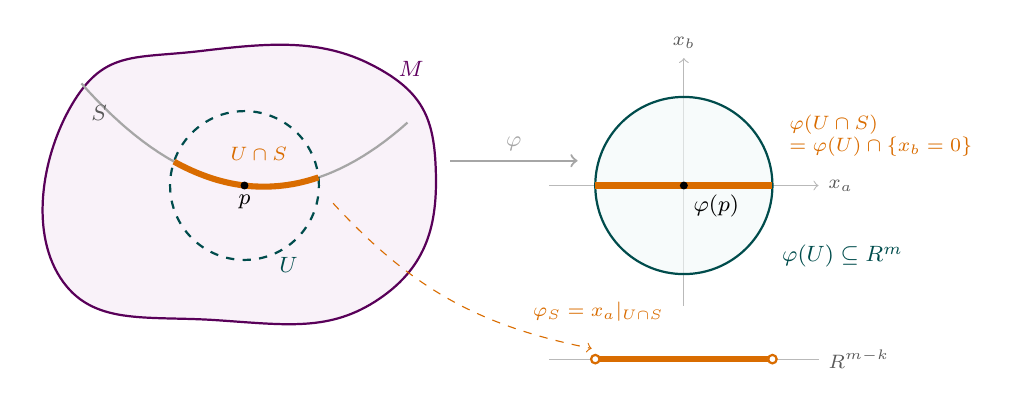
\begin{tikzpicture}[scale=0.9]
\draw[violet!70!black, thick, fill=violet!5] plot[smooth cycle, tension=0.8] coordinates {(-2.6,-1.3) (-2.4,1.2) (-0.6,1.9) (1.8,1.7) (2.7,0.2) (1.9,-1.6) (-0.4,-1.9)};
\node[violet!75!black, font=\footnotesize] at (2.35,1.65) {$M$};
\draw[gray!70, thick] (-2.300,1.440) -- (-2.261,1.396) -- (-2.223,1.354) -- (-2.184,1.311) -- (-2.145,1.270) -- (-2.107,1.229) -- (-2.068,1.189) -- (-2.029,1.150) -- (-1.991,1.111) -- (-1.952,1.073) -- (-1.913,1.035) -- (-1.875,0.998) -- (-1.836,0.962) -- (-1.797,0.927) -- (-1.759,0.892) -- (-1.720,0.857) -- (-1.682,0.824) -- (-1.643,0.791) -- (-1.604,0.759) -- (-1.566,0.727) -- (-1.527,0.696) -- (-1.488,0.666) -- (-1.450,0.636) -- (-1.411,0.607) -- (-1.372,0.579) -- (-1.334,0.551) -- (-1.295,0.524) -- (-1.256,0.498) -- (-1.218,0.472) -- (-1.179,0.447) -- (-1.140,0.423) -- (-1.102,0.399) -- (-1.063,0.376) -- (-1.024,0.354) -- (-0.986,0.332) -- (-0.947,0.311) -- (-0.908,0.291) -- (-0.870,0.271) -- (-0.831,0.252) -- (-0.792,0.233) -- (-0.754,0.215) -- (-0.715,0.198) -- (-0.676,0.182) -- (-0.638,0.166) -- (-0.599,0.151) -- (-0.561,0.136) -- (-0.522,0.123) -- (-0.483,0.109) -- (-0.445,0.097) -- (-0.406,0.085) -- (-0.367,0.074) -- (-0.329,0.063) -- (-0.290,0.053) -- (-0.251,0.044) -- (-0.213,0.035) -- (-0.174,0.028) -- (-0.135,0.020) -- (-0.097,0.014) -- (-0.058,0.008) -- (-0.019,0.002) -- (0.019,-0.002) -- (0.058,-0.006) -- (0.097,-0.010) -- (0.135,-0.012) -- (0.174,-0.014) -- (0.213,-0.016) -- (0.251,-0.016) -- (0.290,-0.016) -- (0.329,-0.016) -- (0.367,-0.014) -- (0.406,-0.012) -- (0.445,-0.010) -- (0.483,-0.007) -- (0.522,-0.003) -- (0.561,0.002) -- (0.599,0.007) -- (0.638,0.013) -- (0.676,0.019) -- (0.715,0.027) -- (0.754,0.035) -- (0.792,0.043) -- (0.831,0.052) -- (0.870,0.062) -- (0.908,0.073) -- (0.947,0.084) -- (0.986,0.095) -- (1.024,0.108) -- (1.063,0.121) -- (1.102,0.135) -- (1.140,0.149) -- (1.179,0.164) -- (1.218,0.180) -- (1.256,0.196) -- (1.295,0.214) -- (1.334,0.231) -- (1.372,0.250) -- (1.411,0.269) -- (1.450,0.288) -- (1.488,0.309) -- (1.527,0.330) -- (1.566,0.351) -- (1.604,0.374) -- (1.643,0.397) -- (1.682,0.420) -- (1.720,0.445) -- (1.759,0.470) -- (1.797,0.495) -- (1.836,0.521) -- (1.875,0.548) -- (1.913,0.576) -- (1.952,0.604) -- (1.991,0.633) -- (2.029,0.663) -- (2.068,0.693) -- (2.107,0.724) -- (2.145,0.755) -- (2.184,0.787) -- (2.223,0.820) -- (2.261,0.854) -- (2.300,0.888); \node[font=\footnotesize, gray!70!black] at (-2.05,1.02) {$S$};
\draw[teal!60!black, thick, dashed] (0,0) circle (1.05); \node[teal!60!black, font=\footnotesize] at (0.62,-1.12) {$U$};
\draw[orange!85!black, line width=2.2pt] (-0.994,0.337) -- (-0.960,0.318) -- (-0.925,0.299) -- (-0.891,0.281) -- (-0.856,0.264) -- (-0.822,0.247) -- (-0.787,0.231) -- (-0.753,0.215) -- (-0.718,0.200) -- (-0.684,0.185) -- (-0.649,0.171) -- (-0.614,0.157) -- (-0.580,0.144) -- (-0.545,0.131) -- (-0.511,0.119) -- (-0.476,0.107) -- (-0.442,0.096) -- (-0.407,0.085) -- (-0.373,0.075) -- (-0.338,0.066) -- (-0.304,0.057) -- (-0.269,0.048) -- (-0.234,0.040) -- (-0.200,0.033) -- (-0.165,0.026) -- (-0.131,0.019) -- (-0.096,0.014) -- (-0.062,0.008) -- (-0.027,0.003) -- (0.007,-0.001) -- (0.042,-0.005) -- (0.076,-0.008) -- (0.111,-0.011) -- (0.146,-0.013) -- (0.180,-0.014) -- (0.215,-0.016) -- (0.249,-0.016) -- (0.284,-0.016) -- (0.318,-0.016) -- (0.353,-0.015) -- (0.387,-0.013) -- (0.422,-0.011) -- (0.456,-0.009) -- (0.491,-0.006) -- (0.526,-0.002) -- (0.560,0.002) -- (0.595,0.006) -- (0.629,0.012) -- (0.664,0.017) -- (0.698,0.023) -- (0.733,0.030) -- (0.767,0.037) -- (0.802,0.045) -- (0.836,0.054) -- (0.871,0.062) -- (0.906,0.072) -- (0.940,0.082) -- (0.975,0.092) -- (1.009,0.103) -- (1.044,0.114);
\fill (0,0) circle (1.6pt) node[below, font=\footnotesize] {$p$};
\node[orange!85!black, font=\scriptsize, anchor=south] at (0.20,0.22) {$U \cap S$};
\draw[->, gray!55] (4.30,0) -- (8.10,0) node[right, font=\scriptsize, text=gray!70!black] {$x_a$}; \draw[->, gray!55] (6.20,-1.7) -- (6.20,1.8) node[above, font=\scriptsize, text=gray!70!black] {$x_b$};
\draw[teal!60!black, thick, fill=teal!5, fill opacity=0.6] (6.20,0) circle (1.25); \node[teal!60!black, font=\footnotesize, anchor=west] at (7.45,-1.0) {$\varphi(U) \subseteq \mathbb{R}^m$};
\draw[orange!85!black, line width=2.2pt] (4.95,0) -- (7.45,0);
\fill (6.20,0) circle (1.6pt) node[below right, font=\footnotesize] {$\varphi(p)$};
\node[orange!85!black, font=\scriptsize, anchor=west, align=left] at (7.55,0.7) {$\varphi(U \cap S)$\\ $= \varphi(U) \cap \{x_b = 0\}$};
\draw[->, thick, gray!70] (2.9,0.35) -- node[above, font=\footnotesize] {$\varphi$} (4.7,0.35);
\draw[gray!55] (4.30,-2.45) -- (8.10,-2.45) node[right, font=\scriptsize, text=gray!70!black] {$\mathbb{R}^{m-k}$};
\draw[orange!85!black, line width=2.2pt] (4.95,-2.45) -- (7.45,-2.45);
\draw[white, fill=white] (4.95,-2.45) circle (1.7pt); \draw[orange!85!black, thick] (4.95,-2.45) circle (1.7pt); \draw[white, fill=white] (7.45,-2.45) circle (1.7pt); \draw[orange!85!black, thick] (7.45,-2.45) circle (1.7pt);
\draw[->, dashed, orange!85!black] (1.25,-0.25) to[bend right=18] node[pos=0.78, above right, font=\scriptsize] {$\varphi_S = x_a|_{U \cap S}$} (4.90,-2.3);
\end{tikzpicture}
